 \section{Tests et résultats}
  Pour vérifier le bon fonctionnement de notre programme, nous avons
  effectué plusieurs tests qui nous ont permis de nous rendre compte de
  plusieurs problèmes.

  \subsection{Tests}
  Nous avons fait plusieurs tests sur différents types de fichiers
  d'entrée. Ces fichiers tests sont disponibles dans le répertoire
  \emph{jeux}. \newline
  \indent Nous avons testé notre programme sur des fichiers vides,
  et différents types de graphes. Des graphes à une seule arête, et des
  graphes générés par le programme \emph{gengraph}: des cliques à 100
  sommets, un chemin à 100 sommets, un graphe complet de 100 sommets, un
  arbre à 100 sommets...

  \subsection{Résultats des tests}
  Ces tests nous ont permis de mettre en avant quelques erreurs de
  programmation que nous avons corrigées mais surtout de trouver des cas
  simples, dont nous avons parlés précédemment, et de voir les limites
  des réductions et de \emph{minisat}.
  \begin{enumerate}
   \item \emph{Circuit Hamiltonien:} Si on lançait la recherche d'un
	 Circuit Hamiltonien sur un graphe complet, à cause du grand
	 nombre de clauses, le temps d'exécution de \emph{minisat}
	 explosait alors qu'il n'y a rien de plus simple à trouver. Cas
	 que nous avons résolu (en ajoutant un cas facile), mais si on
	 enlève une arête à un graphe complet le problème perciste.
   \item \emph{Couverture par sommets:} Si on lance cette réduction sur
	 un graphe de type chemin de taille 100 et que l'on cherche une
	 couverture de sommet de taille 50 ou inférieur (qui n'est pas
	 satisfaisable dans ce denier cas) le temps d'exécution explose
	 littéralement alors qu'en TD, nous avons vu que, pour ce genre
	 de graphe et pour un nombre de sommet paire $n$, la plus petite
	 couverture de sommet est de taille $n/2$ (voir figure
	 \ref{lourd} page \pageref{lourd} en annexe). 
  \end{enumerate}

  \indent Sur des graphes de taille correcte à l'échelle papier (i.e. 4
  ou 5 sommets), les résulats ont tous été concluant. Le résultat de
  l'exécution du programme pour un \emph{Circuit Hamiltonien} (\ref{ham}
  page \pageref{ham}) sur le graphe \ref{graphe1} page \pageref{graphe1} 
  (voir aussi figures \ref{an2} page \pageref{an2} en annexe pour KCol)
  est bien un \emph{Circuit Hamiltonien}.

  \begin{figure}[!ht]
   \begin{center}
    \includegraphics[height=5cm]{images/jeurap.ps}
    \caption{Graphe de test jeurapport.gin .\label{graphe1}}
   \end{center}
  \end{figure}

  \begin{figure}[!ht]
   \begin{center}
    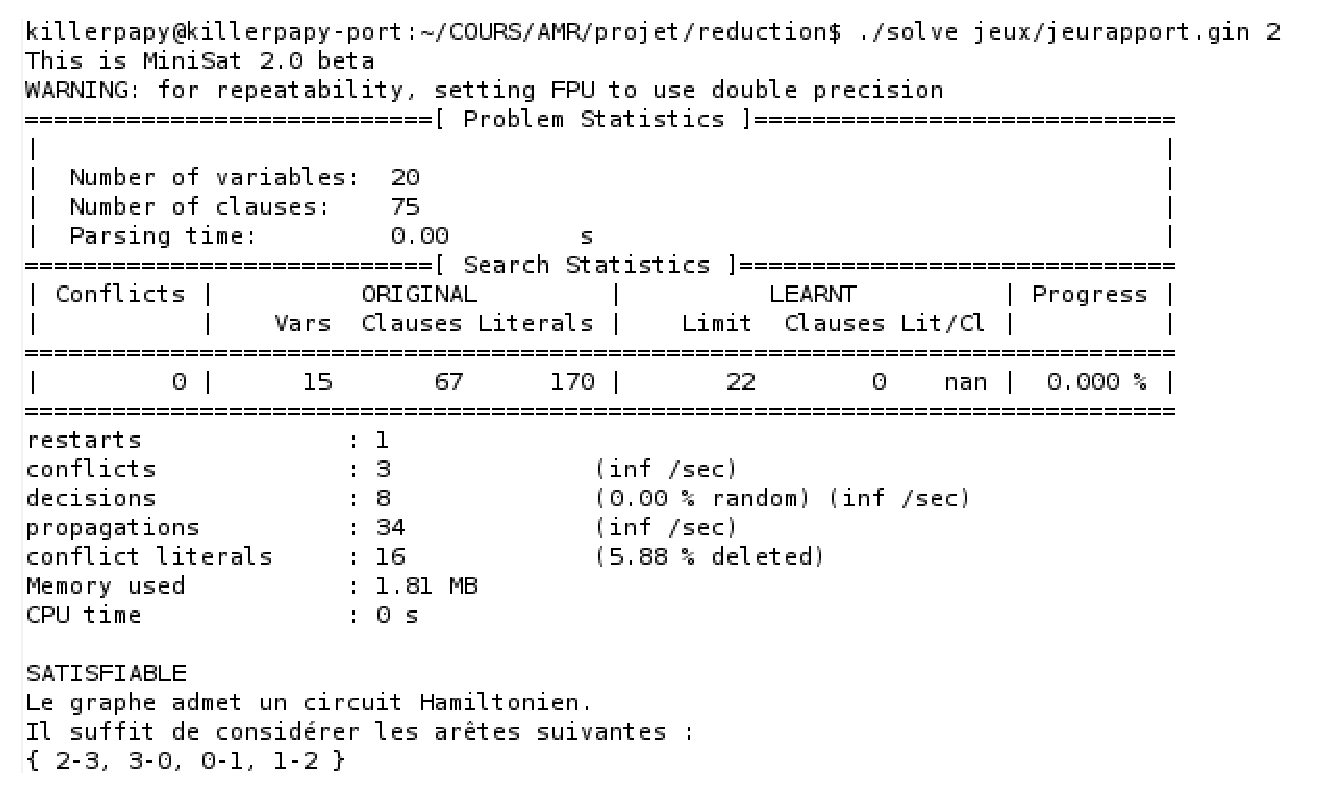
\includegraphics[width=12cm]{images/chemin.eps}
    \caption{\emph{Circuit Hamiltonien} sur le graphe
    \ref{graphe1}.\label{ham}}
   \end{center}
  \end{figure}